\section{问题建模与分析}
\label{sec:problem}

本节先给出任务、航线求解与合理流场集合的模型，再分析粗图下选边的难点，并由此导出方法的三条原则。

\subsection{任务场景与数据}
本文研究航行器携带粗图绕越禁航区时的左右选边。主设置取台湾以东至东海的黑潮区（23°--31°N、121°--129°E），采用HYCOM全球再分析10米深度的1/12°流速场\cite{chassignet2007hycom}，2019年1月1日至2024年8月29日每3天一张快照，共689张；2019--2021年为开发年份，用于标定全部参数，2022--2024年为测试年份，只评价一次。每张快照生成2个任务：起终点相距100--140千米，两点中间设半径15千米的禁航区，只保留粗图上平均流速不低于0.3米/秒的强流任务。航行器携带3天前的1°粗图（格内平均），当天的1/12°场作为真实海流（表\ref{tab:settings}）。为检验结论的适用范围，我们在湾流与阿古拉斯回流区重复了同一流程，并在黑潮区让航行器改带美国国家海洋和大气管理局的近实时融合卫星测高地转流图。

\begin{table}[tb]
\centering
\caption{黑潮主设置的实验设置与参数（其余设置只换海区或粗图来源，参数各自在开发年份标定）。}
\label{tab:settings}
\small
\begin{tabular}{@{}p{0.16\linewidth}p{0.80\linewidth}@{}}
\toprule
项目 & 设置 \\
\midrule
海流数据 & HYCOM 全球海洋再分析（GLBy0.08，实验 93.0），水平分辨率 1/12°，取 10 米深度；23°--31°N、121°--129°E（台湾以东至东海，含黑潮）；2019-01-01 至 2024-08-29 每 3 天 12:00 时一张，共 689 张 \\
任务 & 每张快照抽 2 个：起终点相距 100--140 千米、离岸不少于 20 千米，两点中间设半径 15 千米的禁航区，可从左侧或右侧绕过；只取粗图上任务区平均流速不低于 0.3 米/秒的强流任务；开发 710 个（2019--2021 年），测试 623 个（2022--2024 年） \\
粗图与真实海流 & 航行器带 3 天前的 1° 粗分辨率海流图（下称粗图，格内平均）；真实海流为当天 1/12° 再分析海流场 \\
航行器 & 对水速度 1.0 米/秒；选定一侧后，按真实海流在该侧以最快方式航行 \\
航线求解 & 网格最短路：粗网格求解 8 千米网格、8 个方向；中网格求解 4 千米、16 个方向；细网格求解 2 千米、32 个方向（计算量之比 1 : 8 : 64）；顶流过强的边不可通行 \\
合理流场集合 & 粗图加上由流函数生成的无散误差模态的组合，各点误差大小与相关长度（76 千米）由开发年份标定，组合系数服从标准正态；半径 $r=1.5$（开发年份中包住真实左右航时差的任务占 93\%） \\
合理反例检验 & 在半径 $r$ 的球内对左右航时差做投影梯度上升（梯度沿最快航线累加）；两个方向、半径 1 与 2 各搜一次，其他半径线性插值，每个任务约 71 次中网格求解 \\
观测方式 & 原地停留测流（出发前 2 小时测 12 次）；沿途测流 30 千米或沿途测流 60 千米后可换边；绕行定点测流（去前方 40 千米内反例与粗图差别最大处测量）；上浮取当天 1° 图或上浮取当天 0.5° 图（每次 1 小时）；测流噪声 0.05 米/秒 \\
阈值判据 & 最大后悔值超过 8 小时（开发年份选定）时判定粗图不可信，触发超阈值时保守改选或超阈值时上浮取图，否则按粗图选边 \\
评价指标 & 额外航时 = 实际航时 $-$ 真实更快一侧的航时（小时）；配对差值的 95\% 置信区间按天整组自助重抽样 2000 次 \\
\bottomrule
\end{tabular}

\end{table}

\subsection{航线求解}
给定水平海流场 $\boldsymbol{u}(\boldsymbol{x})$ 与航行器恒定的对水速度 $V = 1.0$ 米/秒，选定绕行一侧 $s \in \{\text{L}, \text{R}\}$（左侧或右侧）后的最快航线由有向图最短路算法求取\cite{dijkstra1959note}。对长度为 $\ell_e$、单位方向为 $\boldsymbol{d}_e$ 的有向边 $e$，记沿边流速分量为 $u_{\parallel} = \boldsymbol{u} \cdot \boldsymbol{d}_e$、垂直边分量为 $u_{\perp} = \|\boldsymbol{u} - u_{\parallel}\boldsymbol{d}_e\|$（边上的流速取两端节点的平均），则航行器的对地速度 $v_{\text{g}}(e)$ 与通行时间 $t(e)$ 为
\begin{equation}
v_{\text{g}}(e) = u_{\parallel} + \sqrt{V^2 - u_{\perp}^2}, \qquad t(e) = \frac{\ell_e}{v_{\text{g}}(e)}.
\label{eq:edge_time}
\end{equation}
当 $|u_{\perp}| \ge V$ 或 $v_{\text{g}}(e) \le 0$ 时该边不可通行。在禁航区左侧或右侧的子图上分别求最短路，得两侧最快航时 $T_{\text{L}}(\boldsymbol{u})$、$T_{\text{R}}(\boldsymbol{u})$ 及左右航时差
\begin{equation}
\Delta T(\boldsymbol{u}) = T_{\text{L}}(\boldsymbol{u}) - T_{\text{R}}(\boldsymbol{u}),
\label{eq:delta_t}
\end{equation}
$\Delta T(\boldsymbol{u}) < 0$ 表示左侧更快。求解分粗网格（8千米、8个方向）、中网格（4千米、16个方向）与细网格（2千米、32个方向）三档，计算量之比为 $1:8:64$。选定一侧后，假设航行器按真实海流 $\boldsymbol{u}_{\text{true}}$ 在该侧以最快方式航行，以便专门评价选边这一顶层决策。

\subsection{合理流场集合}
粗图 $\boldsymbol{u}_0(\boldsymbol{x})$ 的误差成片出现（图\ref{fig:data}），因此我们用空间相关的无散模态而非逐点独立的扰动描述它。以流函数生成误差模态，按历史误差逐点缩放（缩放后近似无散），构造与粗图相容的流场
\begin{equation}
\boldsymbol{u}(\boldsymbol{x}; \boldsymbol{z}) = \boldsymbol{u}_0(\boldsymbol{x}) + \sum_{k=1}^{K} z_k \boldsymbol{m}_k(\boldsymbol{x}), \qquad \boldsymbol{m}_k(\boldsymbol{x}) = \mathbf{S}(\boldsymbol{x})\, \nabla^{\perp}\phi_k(\boldsymbol{x}),
\label{eq:plausible_field}
\end{equation}
其中 $\nabla^{\perp} = (-\partial_y, \partial_x)$，$\{\phi_k\}_{k=1}^{K}$ 为相关长度 $L_{\text{corr}}$ 的高斯相关流函数的前 $K$ 个主模态（保留95\%方差），$\mathbf{S}(\boldsymbol{x})$ 为逐点误差标准差构成的对角矩阵，系数 $\boldsymbol{z} = (z_1, \dots, z_K)^{\top}$ 先验服从标准正态分布。给定半径 $r > 0$，合理流场集合（合理集合）定义为以粗图为中心的不确定集
\begin{equation}
\mathcal{U}(r) = \left\{ \boldsymbol{u}(\boldsymbol{x}; \boldsymbol{z}) \;\middle|\; \|\boldsymbol{z}\|_2 \le r \right\}.
\label{eq:plausible_set}
\end{equation}

\begin{figure}[tb]
\centering
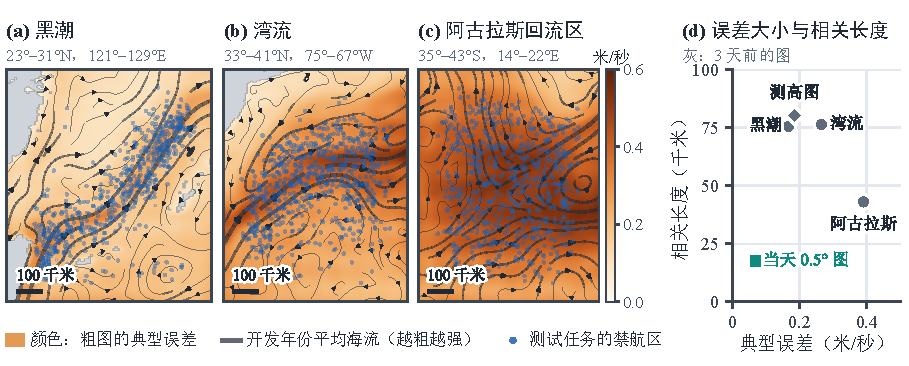
\includegraphics[width=\textwidth]{route3_data}
\caption{三个研究海区与3天前粗图的误差（开发年份）。(a)--(c) 黑潮、湾流与阿古拉斯回流区：底色为3天前1°粗图相对真实海流的典型误差，黑线为平均海流，蓝点为测试任务的禁航区；(d) 各设置所用海流图的典型误差与误差的空间相关长度。3天前的图误差大且成片相关，相关长度与航线尺度相当；当天的0.5°图误差小、相关范围短。}
\label{fig:data}
\end{figure}

\subsection{可选行动与评价指标}
航行器面对粗图有三类行动。一是在同一张粗图上加算，即从粗网格求解改为中网格或细网格求解；在粗图上用细网格求解并选更快一侧，作为基线（按粗图选边）。二是不取新信息、改用其他选边准则，如集合平均选边（在随机抽取的集合成员上选平均航时更短的一侧）或选最大后悔值较小的一侧。三是获取新信息，包括原地停留测流（2小时测12次）、沿途测流30或60千米后再决定是否换边、绕行到指定点测流，以及上浮获取当天的1°或0.5°海流图（每次计1小时）；测得的流速按线性高斯更新修正模态系数。评价指标为额外航时，即实际总航时 $T_{\text{total}}$ 减去真实更快一侧的航时：
\begin{equation}
\mathcal{L} = T_{\text{total}} - \min\left\{ T_{\text{L}}(\boldsymbol{u}_{\text{true}}),\, T_{\text{R}}(\boldsymbol{u}_{\text{true}}) \right\}.
\label{eq:loss}
\end{equation}

\subsection{问题分析}
\label{sec:analysis}
粗图下的选边之所以困难，在于两侧航时接近有两种不同的原因，而观测又各有代价与视野。第一，求解误差与粗图误差混在一起：同一张粗图上，粗网格与细网格求得的左右航时差可相差3.2小时（开发年份的95\%分位数），仅看航时差无法判断该加算还是该观测。第二，粗图误差在空间上大范围相关，各设置的相关长度为43--80千米，与航线尺度相当（图\ref{fig:data}(d)）；一个误差模态就能使整条左侧或右侧通道同时顺流或逆流，因此与粗图同样相容、却要求选另一侧的海流应当普遍存在，“有没有反例”本身难以区分任务的风险高低，需要度量反例会让当前选择多花多少时间。第三，观测的视野与代价不同：就地测流只能看到航线附近，而决定两侧快慢的切变可能远在数十千米之外；上浮取图能同时更新两侧的海流，却要中断航行约1小时。

这三点决定了方法的三条原则（第\ref{sec:method}节）：只在航时差小于求解误差时加算，以排除数值歧义；以最大后悔值而非反例的有无衡量环境歧义；只在最大后悔值超过阈值时付出观测的代价，并优先选用能同时更新两侧的观测。
